\documentclass[11pt,fleqn, openany]{book} % Default font size and left-justified equations

%%%%%%%%%%%%%%%%%%%%%%%%%%%%%%%%%%%%%%%%%
% The Legrand Orange Book
% Structural Definitions File
% Version 2.1 (26/09/2018)
%
% Original author:
% Mathias Legrand (legrand.mathias@gmail.com) with modifications by:
% Vel (vel@latextemplates.com)
% 
% This file was downloaded from:
% http://www.LaTeXTemplates.com
%
% License:
% CC BY-NC-SA 3.0 (http://creativecommons.org/licenses/by-nc-sa/3.0/)
%
%%%%%%%%%%%%%%%%%%%%%%%%%%%%%%%%%%%%%%%%%

%----------------------------------------------------------------------------------------
%	VARIOUS REQUIRED PACKAGES AND CONFIGURATIONS
%----------------------------------------------------------------------------------------

\usepackage[table]{xcolor}

\usepackage{graphicx}
\usepackage{tabularx} % Required for including pictures
\usepackage{pgf,tikz,tkz-tab,eurosym,yhmath, stmaryrd}
\usepackage{pgfplots}
\usepackage{mathrsfs}
\usetikzlibrary{patterns}
\usetikzlibrary{trees}
\graphicspath{{../../Pictures/}}
\usepackage{multicol} 


\usepackage[english]{babel} % English language/hyphenation
\usepackage{icomma}
\usepackage{enumitem} % Customize lists
\setlist{nolistsep, nosep, nolistsep} % Reduce spacing between bullet points and numbered lists

\usepackage{booktabs} % Required for nicer horizontal rules in tables

 % Required for specifying colors by name


\definecolor{ocre}{RGB}{243,102,25} % Define the orange color used for highlighting throughout the book

\usepackage{listings}

\definecolor{codegreen}{rgb}{0,0.6,0}
\definecolor{codegray}{rgb}{0.5,0.5,0.5}
\definecolor{codepurple}{rgb}{0.58,0,0.82}
\definecolor{backcolour}{rgb}{0.95,0.95,0.92}

\lstdefinestyle{mystyle}{
    backgroundcolor=\color{backcolour},   
    commentstyle=\color{codegreen},
    keywordstyle=\color{magenta},
    numberstyle=\tiny\color{codegray},
    stringstyle=\color{codepurple},
    basicstyle=\ttfamily\footnotesize,
    breakatwhitespace=false,         
    breaklines=true,                 
    captionpos=b,                    
    keepspaces=true,                 
    numbers=left,                    
    numbersep=5pt,                  
    showspaces=false,                
    showstringspaces=false,
    showtabs=false,                  
    tabsize=2
}

\lstset{style=mystyle}

%----------------------------------------------------------------------------------------
% Paramétrage XSIM
%----------------------------------------------------------------------------------------

\usepackage[no-files]{xsim}


\DeclareExerciseEnvironmentTemplate{myex}{%
    \textbf{%
      \hypertarget{ex:\ExerciseID}{\sffamily{\ensuremath{\blacktriangleright}} Exercice \GetExerciseProperty{counter} \GetExerciseProperty{subtitle} --}
      \hyperlink{sol:\ExerciseID}{Voir le corrigé}%
    }\par
}{\par\smallskip}

\DeclareExerciseEnvironmentTemplate{mysol}{%
    \textbf{%
      \hypertarget{sol:\ExerciseID}{\sffamily{\ensuremath{\blacktriangleright}} Correction \GetExerciseProperty{counter} --}
      \hyperlink{ex:\ExerciseID}{Voir l'énoncé}%
    }\par
}{\par\medskip}

\xsimsetup{
  exercise/template = myex ,
  solution/template = mysol 
}

%Collection exercices

\DeclareExerciseTagging{topic}

\xsimsetup{collect}

%----------------------------------------------------------------------------------------
% SYMBOLES
%----------------------------------------------------------------------------------------

\newcommand\imCMsym[4][\mathord]{%
  \DeclareFontFamily{U} {#2}{}
  \DeclareFontShape{U}{#2}{m}{n}{
    <-6> #25
    <6-7> #26
    <7-8> #27
    <8-9> #28
    <9-10> #29
    <10-12> #210
    <12-> #212}{}
  \DeclareSymbolFont{CM#2} {U} {#2}{m}{n}
  \DeclareMathSymbol{#4}{#1}{CM#2}{#3}
}
\newcommand\alsoimCMsym[4][\mathord]{\DeclareMathSymbol{#4}{#1}{CM#2}{#3}}

\imCMsym{cmmi}{124}{\CMjmath}

\newcommand{\Oij}{(O\,;\,\vec{\imath}\,,\, \vec{\CMjmath} )}
\newcommand{\Oijk}{(O\,;\,\vec{\imath}\,,\, \vec{\CMjmath}\,,\,\vec{k})}

\newcommand\e{\mathrm{e}}
\newcommand\R{\mathbb{R}}
\newcommand\N{\mathbb{N}}


%----------------------------------------------------------------------------------------
%	MARGINS
%----------------------------------------------------------------------------------------

\usepackage{geometry} % Required for adjusting page dimensions and margins

\geometry{
	paper=a4paper, % Paper size, change to letterpaper for US letter size
	top=3cm, % Top margin
	bottom=3cm, % Bottom margin
	left=2cm, % Left margin
	right=2cm, % Right margin
	headheight=14pt, % Header height
	footskip=1.4cm, % Space from the bottom margin to the baseline of the footer
	headsep=10pt, % Space from the top margin to the baseline of the header
	%showframe, % Uncomment to show how the type block is set on the page
}

\setlength{\parindent}{0pt}
\parskip=5pt



%----------------------------------------------------------------------------------------
%	FONTS
%----------------------------------------------------------------------------------------

\usepackage{avant} % Use the Avantgarde font for headings
\usepackage{times} % Use the Times font for headings
\usepackage{mathptmx} % Use the Adobe Times Roman as the default text font together with math symbols from the Sym­bol, Chancery and Com­puter Modern fonts

%\usepackage{microtype} % Slightly tweak font spacing for aesthetics
%\usepackage[utf8]{inputenc} % Required for including letters with accents
\usepackage[T1]{fontenc} % Use 8-bit encoding that has 256 glyphs

%----------------------------------------------------------------------------------------
%	BIBLIOGRAPHY AND INDEX
%----------------------------------------------------------------------------------------

\usepackage[style=numeric,citestyle=numeric,sorting=nyt,sortcites=true,autopunct=true,babel=hyphen,hyperref=true,abbreviate=false,backref=true,backend=biber]{biblatex}
\addbibresource{bibliography.bib} % BibTeX bibliography file
\defbibheading{bibempty}{}

\usepackage{calc} % For simpler calculation - used for spacing the index letter headings correctly
\usepackage{makeidx} % Required to make an index
\makeindex % Tells LaTeX to create the files required for indexing

%----------------------------------------------------------------------------------------
%	MAIN TABLE OF CONTENTS
%----------------------------------------------------------------------------------------

\usepackage{titletoc} % Required for manipulating the table of contents

\contentsmargin{0cm} % Removes the default margin

% Part text styling (this is mostly taken care of in the PART HEADINGS section of this file)
\titlecontents{part}
	[0cm] % Left indentation
	{\addvspace{20pt}\bfseries} % Spacing and font options for parts
	{}
	{}
	{}

% Chapter text styling
\titlecontents{chapter}
	[1.25cm] % Left indentation
	{\addvspace{12pt}\large\sffamily\bfseries} % Spacing and font options for chapters
	{\color{ocre!60}\contentslabel[\Large\thecontentslabel]{1.25cm}\color{ocre}} % Formatting of numbered sections of this type
	{\color{ocre}} % Formatting of numberless sections of this type
	{\color{ocre!60}\normalsize\;\titlerule*[.5pc]{.}\;\thecontentspage} % Formatting of the filler to the right of the heading and the page number

% Section text styling
\titlecontents{section}
	[1.25cm] % Left indentation
	{\addvspace{3pt}\sffamily\bfseries} % Spacing and font options for sections
	{\contentslabel[\thecontentslabel]{1.25cm}} % Formatting of numbered sections of this type
	{} % Formatting of numberless sections of this type
	{\hfill\color{black}\thecontentspage} % Formatting of the filler to the right of the heading and the page number

% Subsection text styling
\titlecontents{subsection}
	[1.25cm] % Left indentation
	{\addvspace{1pt}\sffamily\small} % Spacing and font options for subsections
	{\contentslabel[\thecontentslabel]{1.25cm}} % Formatting of numbered sections of this type
	{} % Formatting of numberless sections of this type
	{\ \titlerule*[.5pc]{.}\;\thecontentspage} % Formatting of the filler to the right of the heading and the page number

% Figure text styling
\titlecontents{figure}
	[1.25cm] % Left indentation
	{\addvspace{1pt}\sffamily\small} % Spacing and font options for figures
	{\thecontentslabel\hspace*{1em}} % Formatting of numbered sections of this type
	{} % Formatting of numberless sections of this type
	{\ \titlerule*[.5pc]{.}\;\thecontentspage} % Formatting of the filler to the right of the heading and the page number

% Table text styling
\titlecontents{table}
	[1.25cm] % Left indentation
	{\addvspace{1pt}\sffamily\small} % Spacing and font options for tables
	{\thecontentslabel\hspace*{1em}} % Formatting of numbered sections of this type
	{} % Formatting of numberless sections of this type
	{\ \titlerule*[.5pc]{.}\;\thecontentspage} % Formatting of the filler to the right of the heading and the page number

%----------------------------------------------------------------------------------------
%	MINI TABLE OF CONTENTS IN PART HEADS
%----------------------------------------------------------------------------------------

% Chapter text styling
\titlecontents{lchapter}
	[0em] % Left indentation
	{\addvspace{15pt}\large\sffamily\bfseries} % Spacing and font options for chapters
	{\color{ocre}\contentslabel[\Large\thecontentslabel]{1.25cm}\color{ocre}} % Chapter number
	{}  
	{\color{ocre}\normalsize\sffamily\bfseries\;\titlerule*[.5pc]{.}\;\thecontentspage} % Page number

% Section text styling
\titlecontents{lsection}
	[0em] % Left indentation
	{\sffamily\small} % Spacing and font options for sections
	{\contentslabel[\thecontentslabel]{1.25cm}} % Section number
	{}
	{}

% Subsection text styling (note these aren't shown by default, display them by searchings this file for tocdepth and reading the commented text)
\titlecontents{lsubsection}
	[.5em] % Left indentation
	{\sffamily\footnotesize} % Spacing and font options for subsections
	{\contentslabel[\thecontentslabel]{1.25cm}}
	{}
	{}

%----------------------------------------------------------------------------------------
%	HEADERS AND FOOTERS
%----------------------------------------------------------------------------------------


\usepackage{fancyhdr} % Required for header and footer configuration

\pagestyle{fancy}
\renewcommand{\chaptermark}[1]{\markboth{\sffamily\normalsize\bfseries\ \thechapter.\ #1}{}} % Chapter text font settings
\renewcommand{\sectionmark}[1]{\markright{\sffamily\normalsize\thesection\hspace{5pt}#1}{}} % Section text font settings
\fancyhf{} \fancyhead[LE,RO]{\sffamily\normalsize\thepage} % Font setting for the page number in the header
\fancyhead[LO]{\rightmark} % Print the nearest section name on the left side of odd pages
\fancyhead[RE]{\leftmark} % Print the current chapter name on the right side of even pages

\fancyfoot[L]{Jason LAPEYRONNIE}
\fancyfoot[R]{\href{http://mathoutils.fr}{http://mathoutils.fr}} % Uncomment to include a footer

\renewcommand{\headrulewidth}{0.5pt} % Thickness of the rule under the header
\renewcommand{\footrulewidth}{0.5pt} % Thickness of the rule under the header

\fancypagestyle{plain}{% Style for when a plain pagestyle is specified
	\fancyhead{}\renewcommand{\headrulewidth}{0pt}%
}

% Removes the header from odd empty pages at the end of chapters
\makeatletter
\renewcommand{\cleardoublepage}{
\clearpage\ifodd\c@page\else
\hbox{}
\vspace*{\fill}
\thispagestyle{empty}
\newpage
\fi}

%----------------------------------------------------------------------------------------
%	THEOREM STYLES
%----------------------------------------------------------------------------------------

\usepackage{amsmath,amsfonts,amssymb,amsthm} % For math equations, theorems, symbols, etc

\newcommand{\intoo}[2]{\mathopen{]}#1\,;#2\mathclose{[}}
\newcommand{\ud}{\mathop{\mathrm{{}d}}\mathopen{}}
\newcommand{\intff}[2]{\mathopen{[}#1\,;#2\mathclose{]}}
\renewcommand{\qedsymbol}{$\blacksquare$}
\newtheorem{notation}{Notation}[section]

% Boxed/framed environments
\newtheoremstyle{ocrenumbox}% Theorem style name
{0pt}% Space above
{0pt}% Space below
{\normalfont}% Body font
{}% Indent amount
{\small\bf\sffamily\color{ocre}}% Theorem head font
{\;:\;}% Punctuation after theorem head
{0.25em}% Space after theorem head
{\small\sffamily\color{ocre}\thmname{#1}\nobreakspace\thmnumber{\@ifnotempty{#1}{}\@upn{#2}}% Theorem text (e.g. Theorem 2.1)
\thmnote{\nobreakspace\the\thm@notefont\sffamily\bfseries\color{black}---\nobreakspace#3}} % Optional theorem note

\newtheoremstyle{blacknumex}% Theorem style name
{5pt}% Space above
{10pt}% Space below
{\normalfont}% Body font
{} % Indent amount
{\small\bf\sffamily}% Theorem head font
{\;:\;}% Punctuation after theorem head
{0.25em}% Space after theorem head
{\small\sffamily{\tiny\ensuremath{\blacksquare}}\nobreakspace\thmname{#1}\nobreakspace\thmnumber{\@ifnotempty{#1}{}\@upn{#2}}% Theorem text (e.g. Theorem 2.1)
\thmnote{\nobreakspace\the\thm@notefont\sffamily\bfseries---\nobreakspace#3}}% Optional theorem note

\newtheoremstyle{blacknumexo}% Theorem style name
{15pt}% Space above
{10pt}% Space below
{\normalfont}% Body font
{} % Indent amount
{\small\bf\sffamily}% Theorem head font
{}% Punctuation after theorem head
{0.5em}% Space after theorem head
{\small\sffamily{\ensuremath{\blacktriangleright}}\nobreakspace\thmname{#1}\nobreakspace\thmnumber{\@ifnotempty{#1}{}\@upn{#2}}% Theorem text (e.g. Theorem 2.1)
\thmnote{\nobreakspace\the\thm@notefont\sffamily\bfseries---\nobreakspace#3} \\}% Optional theorem note



\newtheoremstyle{blacknumbox} % Theorem style name
{0pt}% Space above
{5pt}% Space below
{}% Body font
{}% Indent amount
{\large\bf\sffamily}% Theorem head font
{\;:\;}% Punctuation after theorem head
{0.25em}% Space after theorem head
{\small\sffamily\thmname{#1}\nobreakspace\thmnumber{\@ifnotempty{#1}{}\@upn{#2}}% Theorem text (e.g. Theorem 2.1)
\thmnote{\nobreakspace\the\thm@notefont\sffamily\bfseries---\nobreakspace#3}}% Optional theorem note

% Non-boxed/non-framed environments
\newtheoremstyle{ocrenum}% Theorem style name
{5pt}% Space above
{5pt}% Space below
{\normalfont}% Body font
{}% Indent amount
{\small\bf\sffamily\color{ocre}}% Theorem head font
{\;:\;}% Punctuation after theorem head
{0.25em}% Space after theorem head
{\small\sffamily\color{ocre}\thmname{#1}\nobreakspace\thmnumber{\@ifnotempty{#1}{}\@upn{#2}}% Theorem text (e.g. Theorem 2.1)
\thmnote{\nobreakspace\the\thm@notefont\sffamily\bfseries\color{black}---\nobreakspace#3}} % Optional theorem note
\makeatother

% Defines the theorem text style for each type of theorem to one of the three styles above
\newcounter{dummy} 
\newcounter{thm}
\newcounter{correction}
\newcounter{qst}
\theoremstyle{ocrenumbox}
\newtheorem{theoremeT}[dummy]{Théorème}
\newtheorem{exerciseT}{Propriété}
\newtheorem{principeT}{Principe}
\theoremstyle{blacknumex}
\newtheorem{exampleT}{Exemple}
\theoremstyle{blacknumexo}
\newtheorem{exo}[thm]{Exercice}
\newtheorem{corr}[correction]{Correction}
\newtheorem{quest}[qst]{Question}
\theoremstyle{blacknumbox}
\newtheorem{vocabulary}{Vocabulary}[section]
\newtheorem{definitionT}{Définition}
\newtheorem{corollaryT}[dummy]{Corollary}
\theoremstyle{ocrenum}
\newtheorem{proofT}[dummy]{Démonstration}


%----------------------------------------------------------------------------------------
%	DEFINITION OF COLORED BOXES
%----------------------------------------------------------------------------------------

\RequirePackage[framemethod=default]{mdframed} % Required for creating the theorem, definition, exercise and corollary boxes

% Theorem box
\newmdenv[skipabove=7pt,
skipbelow=7pt,
backgroundcolor=black!5,
linecolor=ocre,
innerleftmargin=5pt,
innerrightmargin=5pt,
innertopmargin=10pt,
leftmargin=0cm,
rightmargin=0cm,
innerbottommargin=5pt]{tBox}

%Proposition box	  
\newmdenv[skipabove=7pt,
skipbelow=7pt,
rightline=false,
leftline=true,
topline=false,
bottomline=false,
backgroundcolor=ocre!10,
linecolor=ocre,
innerleftmargin=5pt,
innerrightmargin=5pt,
innertopmargin=10pt,
innerbottommargin=3pt,
leftmargin=0cm,
rightmargin=0cm,
linewidth=4pt]{eBox}	

% Definition box
\newmdenv[skipabove=7pt,
backgroundcolor=ocre!4,
skipbelow=7pt,
rightline=false,
leftline=true,
topline=false,
bottomline=false,
linecolor=ocre,
innerleftmargin=5pt,
innerrightmargin=5pt,
innertopmargin=10pt,
leftmargin=0cm,
rightmargin=0cm,
linewidth=4pt,
innerbottommargin=5pt]{dBox}	

% Corollary box
\newmdenv[skipabove=7pt,
skipbelow=7pt,
rightline=false,
leftline=true,
topline=false,
bottomline=false,
linecolor=gray,
backgroundcolor=black!5,
innerleftmargin=5pt,
innerrightmargin=5pt,
innertopmargin=5pt,
leftmargin=0cm,
rightmargin=0cm,
linewidth=4pt,
innerbottommargin=5pt]{cBox}

\newmdenv[skipabove=7pt,
skipbelow=7pt,
backgroundcolor=black!5,
innerleftmargin=5pt,
topline=false,
bottomline=false,
rightline=false,
leftline=false,
innerrightmargin=5pt,
innertopmargin=5pt,
leftmargin=0cm,
rightmargin=0cm,
innerbottommargin=5pt]{xBox}

% Creates an environment for each type of theorem and assigns it a theorem text style from the "Theorem Styles" section above and a colored box from above
\newenvironment{theorem}{\begin{tBox}\begin{theoremeT}}{\end{theoremeT}\end{tBox}}

\newenvironment{exo2}{\noindent \begin{exo}\item\relax \noindent \begin{eBox}\item\relax}{\end{eBox}\end{exo}}


\newenvironment{proposition}{\begin{eBox}\begin{exerciseT}}{\hfill{\color{ocre}}\end{exerciseT}\end{eBox}}		

\newenvironment{principe}{\begin{eBox}\begin{principeT}}{\hfill{\color{ocre}}\end{principeT}\end{eBox}}	
		  
\newenvironment{definition}{\begin{dBox}\begin{definitionT}}{\end{definitionT}\end{dBox}}	

\newenvironment{example}{\begin{xBox}\begin{exampleT}}{\hfill{\tiny\ensuremath{\blacksquare}}\end{exampleT}\end{xBox}}

\newenvironment{demonstration}{\begin{proofT}}{\hfill{\tiny\ensuremath{\square}}\end{proofT}}		
\newenvironment{corollary}{\begin{cBox}\begin{corollaryT}}{\end{corollaryT}\end{cBox}}	

%----------------------------------------------------------------------------------------
%	REMARK ENVIRONMENT
%----------------------------------------------------------------------------------------

\newenvironment{remark}{\par\vspace{5pt}\small % Vertical white space above the remark and smaller font size
\begin{list}{}{
\leftmargin=25pt % Indentation on the left
\rightmargin=15pt}\item\ignorespaces % Indentation on the right
\makebox[-2.5pt]{\begin{tikzpicture}[overlay]
\node[draw=ocre!60,line width=1pt,circle,fill=ocre!25,font=\sffamily\bfseries,inner sep=2pt,outer sep=0pt] at (-15pt,0pt){\textcolor{ocre}{R}};\end{tikzpicture}} % Orange R in a circle
\advance\baselineskip -1pt}{\end{list}\vskip5pt} % Tighter line spacing and white space after remark

%----------------------------------------------------------------------------------------
%	SECTION NUMBERING IN THE MARGIN
%----------------------------------------------------------------------------------------

\makeatletter
\renewcommand{\@seccntformat}[1]{\llap{\textcolor{ocre}{\csname the#1\endcsname}\hspace{1em}}}                    
\renewcommand{\section}{\@startsection{section}{1}{\z@}
{-4ex \@plus -1ex \@minus -.4ex}
{1ex \@plus.2ex }
{\normalfont\LARGE\sffamily\bfseries}}
\renewcommand{\subsection}{\@startsection {subsection}{2}{\z@}
{-3ex \@plus -0.1ex \@minus -.4ex}
{0.5ex \@plus.2ex }
{\normalfont\sffamily\bfseries}}
\renewcommand{\subsubsection}{\@startsection {subsubsection}{3}{\z@}
{-2ex \@plus -0.1ex \@minus -.2ex}
{.2ex \@plus.2ex }
{\normalfont\small\sffamily\bfseries}}                        
\renewcommand\paragraph{\@startsection{paragraph}{4}{\z@}
{-2ex \@plus-.2ex \@minus .2ex}
{.1ex}
{\normalfont\small\sffamily\bfseries}}

%----------------------------------------------------------------------------------------
%	PART HEADINGS
%----------------------------------------------------------------------------------------

% Numbered part in the table of contents
\newcommand{\@mypartnumtocformat}[2]{%
	\setlength\fboxsep{0pt}%
	\noindent\colorbox{ocre!20}{\strut\parbox[c][.7cm]{\ecart}{\color{ocre!70}\Large\sffamily\bfseries\centering#1}}\hskip\esp\colorbox{ocre!40}{\strut\parbox[c][.7cm]{\linewidth-\ecart-\esp}{\Large\sffamily\centering#2}}%
}

% Unnumbered part in the table of contents
\newcommand{\@myparttocformat}[1]{%
	\setlength\fboxsep{0pt}%
	\noindent\colorbox{ocre!40}{\strut\parbox[c][.7cm]{\linewidth}{\Large\sffamily\centering#1}}%
}

\newlength\esp
\setlength\esp{4pt}
\newlength\ecart
\setlength\ecart{1.2cm-\esp}
\newcommand{\thepartimage}{}%
\newcommand{\partimage}[1]{\renewcommand{\thepartimage}{#1}}%
\def\@part[#1]#2{%
\ifnum \c@secnumdepth >-2\relax%
\refstepcounter{part}%
\addcontentsline{toc}{part}{\texorpdfstring{\protect\@mypartnumtocformat{\thepart}{#1}}{\partname~\thepart\ ---\ #1}}
\else%
\addcontentsline{toc}{part}{\texorpdfstring{\protect\@myparttocformat{#1}}{#1}}%
\fi%
\startcontents%
\markboth{}{}%
{\thispagestyle{empty}%
\begin{tikzpicture}[remember picture,overlay]%
\node at (current page.north west){\begin{tikzpicture}[remember picture,overlay]%	
\fill[ocre!20](0cm,0cm) rectangle (\paperwidth,-\paperheight);
\node[anchor=north] at (4cm,-3.25cm){\color{ocre!40}\fontsize{220}{100}\sffamily\bfseries\thepart}; 
\node[anchor=south east] at (\paperwidth-1cm,-\paperheight+1cm){\parbox[t][][t]{8.5cm}{
\printcontents{l}{0}{\setcounter{tocdepth}{1}}% The depth to which the Part mini table of contents displays headings; 0 for chapters only, 1 for chapters and sections and 2 for chapters, sections and subsections
}};
\node[anchor=north east] at (\paperwidth-1.5cm,-3.25cm){\parbox[t][][t]{15cm}{\strut\raggedleft\color{white}\fontsize{30}{30}\sffamily\bfseries#2}};
\end{tikzpicture}};
\end{tikzpicture}}%
\@endpart}
\def\@spart#1{%
\startcontents%
\phantomsection
{\thispagestyle{empty}%
\begin{tikzpicture}[remember picture,overlay]%
\node at (current page.north west){\begin{tikzpicture}[remember picture,overlay]%	
\fill[ocre!20](0cm,0cm) rectangle (\paperwidth,-\paperheight);
\node[anchor=north east] at (\paperwidth-1.5cm,-3.25cm){\parbox[t][][t]{15cm}{\strut\raggedleft\color{white}\fontsize{30}{30}\sffamily\bfseries#1}};
\end{tikzpicture}};
\end{tikzpicture}}
\addcontentsline{toc}{part}{\texorpdfstring{%
\setlength\fboxsep{0pt}%
\noindent\protect\colorbox{ocre!40}{\strut\protect\parbox[c][.7cm]{\linewidth}{\Large\sffamily\protect\centering #1\quad\mbox{}}}}{#1}}%
\@endpart}
\def\@endpart{\vfil\newpage
\if@twoside
\if@openright
\null
\thispagestyle{empty}%
\newpage
\fi
\fi
\if@tempswa
\twocolumn
\fi}

%----------------------------------------------------------------------------------------
%	CHAPTER HEADINGS
%----------------------------------------------------------------------------------------

% A switch to conditionally include a picture, implemented by Christian Hupfer
\newif\ifusechapterimage
\usechapterimagetrue
\newcommand{\thechapterimage}{}%
\newcommand{\chapterimage}[1]{\ifusechapterimage\renewcommand{\thechapterimage}{#1}\fi}%
\newcommand{\autodot}{.}
\def\@makechapterhead#1{%
{\parindent \z@ \raggedright \normalfont
\ifnum \c@secnumdepth >\m@ne
\if@mainmatter
\begin{tikzpicture}[remember picture,overlay]
\node at (current page.north west)
{\begin{tikzpicture}[remember picture,overlay]
\node[anchor=north west,inner sep=0pt] at (0,0) {\ifusechapterimage\includegraphics[width=\paperwidth]{\thechapterimage}\fi};
\draw[anchor=west] (\Gm@lmargin,-3cm) node [line width=2pt,rounded corners=15pt,draw=ocre,fill=white,fill opacity=0.5,inner sep=15pt]{\strut\makebox[22cm]{}};
\draw[anchor=west] (\Gm@lmargin+.3cm,-3cm) node {\huge\sffamily\bfseries\color{black}\thechapter\autodot~#1\strut};
\end{tikzpicture}};
\end{tikzpicture}
\else
\begin{tikzpicture}[remember picture,overlay]
\node at (current page.north west)
{\begin{tikzpicture}[remember picture,overlay]
\node[anchor=north west,inner sep=0pt] at (0,0) {\ifusechapterimage\includegraphics[width=\paperwidth]{\thechapterimage}\fi};
\draw[anchor=west] (\Gm@lmargin,-3cm) node [line width=2pt,rounded corners=15pt,draw=ocre,fill=white,fill opacity=0.5,inner sep=15pt]{\strut\makebox[22cm]{}};
\draw[anchor=west] (\Gm@lmargin+.3cm,-3cm) node {\huge\sffamily\bfseries\color{black}#1\strut};
\end{tikzpicture}};
\end{tikzpicture}
\fi\fi\par\vspace*{50\p@}}}

%-------------------------------------------

\def\@makeschapterhead#1{%
\begin{tikzpicture}[remember picture,overlay]
\node at (current page.north west)
{\begin{tikzpicture}[remember picture,overlay]
\node[anchor=north west,inner sep=0pt] at (0,0) {\ifusechapterimage\includegraphics[width=\paperwidth]{\thechapterimage}\fi};
\draw[anchor=west] (\Gm@lmargin,-3cm) node [line width=2pt,rounded corners=15pt,draw=ocre,fill=white,fill opacity=0.5,inner sep=15pt]{\strut\makebox[22cm]{}};
\draw[anchor=west] (\Gm@lmargin+.3cm,-3cm) node {\huge\sffamily\bfseries\color{black}#1\strut};
\end{tikzpicture}};
\end{tikzpicture}
\par\vspace*{50\p@}}
\makeatother

%----------------------------------------------------------------------------------------
%	LINKS
%----------------------------------------------------------------------------------------

\usepackage{hyperref}
\hypersetup{hidelinks,backref=true,pagebackref=true,hyperindex=true,colorlinks=false,breaklinks=true,urlcolor=ocre,bookmarks=true,bookmarksopen=false}

\usepackage{bookmark}
\bookmarksetup{
open,
numbered,
addtohook={%
\ifnum\bookmarkget{level}=0 % chapter
\bookmarksetup{bold}%
\fi
\ifnum\bookmarkget{level}=-1 % part
\bookmarksetup{color=ocre,bold}%
\fi
}
}

\renewcommand*\thesection{\arabic{section}}

\newcommand*{\coord}[3]{% 
  \ensuremath{\overrightarrow{#1}\, 
    \begin{pmatrix} 
      #2\\ 
      #3 
    \end{pmatrix}}}
    
  \newcommand*{\coordb}[2]{% 
  \ensuremath{ 
    \begin{pmatrix} 
      #1\\ 
      #2 
    \end{pmatrix}}}

\newcommand*{\coorde}[4]{% 
  \renewcommand{\arraystretch}{1}\ensuremath{\overrightarrow{#1}\, 
    \begin{pmatrix} 
      #2\\ 
      #3 \\
      #4
    \end{pmatrix}}}    
  \newcommand*{\coordbe}[3]{% 
 \renewcommand{\arraystretch}{1} \ensuremath{ 
    \begin{pmatrix} 
      #1\\ 
      #2 \\
      #3
    \end{pmatrix}}}  
    
\newcommand{\Card}{\mathrm{Card}}



\begin{document}

\chapterimage{../../Pictures/background}

\chapter{Cours : Comparaisons des limites}

\section{Théorèmes de comparaison et d'encadrement}

\subsection{Théorèmes de comparaison}

\begin{theorem}[Théorème de comparaison 1]On considère deux suites réelles $(u_n)$ et $(v_n)$. On suppose qu'il existe un entier naturel $N$ tel que, pour tout entier $n \geqslant N$, on a $u_n \leqslant v_n$. 

Si  $\displaystyle \lim_{n \to +\infty} u_n = +\infty$, alors  $\displaystyle \lim_{n \to +\infty} v_n = +\infty $.\end{theorem}

Il n'y a rien de surprenant ici, si l'on fait preuve d'un brin de logique. Si une suite est plus grande qu'une suite qui devient plus grande que n'importe quel réel, alors elle devient elle-même plus grande que n'importe quel réel.

\begin{demonstration} Soit $N$ un entier naturel tel que, pour tout $n\geqslant N$, $u_n \leqslant v_n$.

\vskip50pt

\end{demonstration}

\begin{example} Pour tout entier naturel $n$, on pose $v_n=n+\cos (n)$.

\vskip30pt
\end{example}


\begin{theorem}[Théorème de comparaison 2]On considère deux suites réelles $(u_n)$ et $(v_n)$. On suppose qu'il existe un entier naturel $N$ tel que, pour tout entier $n \geqslant N$, on a $u_n \geqslant v_n$. 

Si  $\displaystyle \lim_{n \to +\infty} u_n = -\infty$, alors  $\displaystyle \lim_{n \to +\infty} v_n = -\infty $.\end{theorem}

Il s'agit d'une version similaire au premier théorème de comparaison : une suite plus petite qu'une suite qui tend vers $-\infty$ tend également vers $-\infty$. La démonstration de ce résultat est d'ailleurs tout à fait similaire.

\begin{example}Pour tout entier naturel $n$, on pose $v_n=(\cos(n)-2)n$.

\vskip30pt \end{example}

Dans les deux exemples précédents, il était possible d'encadrer les termes de la suite dont on souhaitait déterminer la limite. Ainsi, pour ce dernier exemple, on aurait pu préciser que, pour tout entier naturel $n$, $-3n \leqslant v_n \leqslant -n$. Cet encadrement est tout à fait juste mais seule l'une de ces inégalités (en l'occurrence, celle de droite), permet d'établir la limite de la suite. Être supérieur à une suite qui tend vers $-\infty$ n'a rien d'incroyable, alors qu'être inférieur à une telle suite est plus « exceptionnel ».

Toutefois, le prochain théorème ne pourra pas se contenter d'une simple inégalité...

\subsection{Théorème d'encadrement}

\begin{theorem}On considère trois suites $(u_n)$, $(v_n)$ et $(w_n)$. On suppose qu'il existe un entier naturel $N$ tel que, pour tout entier $n\geqslant N$, on a $u_n \leqslant v_n \leqslant w_n$.

Si les suites $(u_n)$ et $(w_n)$ sont convergentes et sont \textbf{de même limite} $\ell$, alors la suite $(v_n)$ est également convergente et $\displaystyle\lim_{n\to+\infty}v_n=\ell$.\end{theorem}



\textbf{Illustration} : Sur l'exemple suivant, trois suites $(u_n)$, $(v_n)$ et $(w_n)$ sont représentées. Pour tout entier naturel $n$, $u_n \leqslant v_n \leqslant w_n$. Si l'on sait que $(u_n)$ et $(w_n)$ sont convergentes de même limite, on en déduit la convergence et limite de la suite $(v_n)$.

\begin{center}
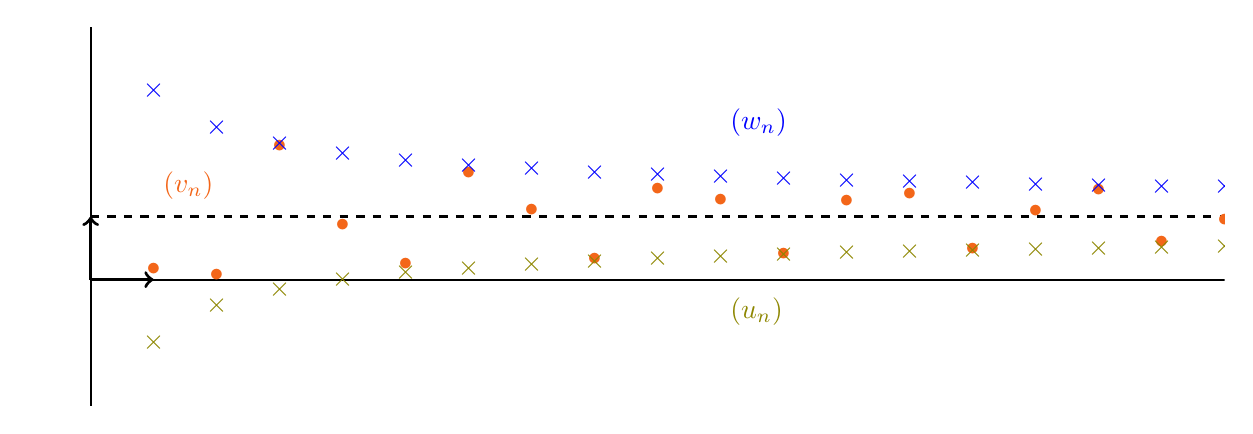
\begin{tikzpicture}[scale=0.8]
\clip (-1,-2) rectangle (18,4);
\draw [thick] (0,0)--(22,0);
\draw [thick] (0,-2)--(0,28);
\draw [->, very thick] (0,0)--(1,0);
\draw [->,very thick] (0,0)--(0,1);
\draw [very thick, dashed, domain = 0:22] plot (\x,1);
\foreach \k in {1,2,...,21} {\draw [very thick, ocre] (\k,{1+2*cos(2*deg(\k))/sqrt(\k)}) node {$\bullet$};}
\foreach \k in {1,2,...,21} {\draw [very thick, blue] (\k,{1+2/sqrt(\k)}) node {$\times$};}
\foreach \k in {1,2,...,21} {\draw [very thick, olive] (\k,{1-2/sqrt(\k)}) node {$\times$};}

\draw [blue] (10,2.5) node[right] {$(w_n)$};
\draw [olive] (10,-0.5) node[right] {$(u_n)$};
\draw [ocre] (1,1.5) node[right] {$(v_n)$};

\end{tikzpicture}
\end{center}

Ce théorème est également appelé « théorème des gendarmes ». Les suites $(w_n)$ et $(u_n)$ jouent ici le rôle des gendarmes qui encerclent leur cible, la suite $(v_n)$. Peu à peu, les gendarmes se dirigent vers la prison. La suite $(v_n)$, encerclée, n'a d'autre choix que de les suivre. D'autres noms plus ou moins évocateurs sont donnés à ce théorème : théorème des carabiniers ou théorème du sandwich par exemple.

Remarquons que ce théorème est avant tout un théorème qui établit la convergence d'une suite ! Encadrer les termes d'une suite par ceux de deux suites convergentes ne garantit pas la convergence de la suite encadrée. 

\textbf{Si toutefois, la suite est convergente}, alors la limite de cette suite est comprise (au sens large) entre les limites des suites encadrantes. La convergence doit cependant être établi au préalable.

\begin{demonstration} Notons $N$ l'entier à partir duquel on a, pour tout $n\geqslant N$, $u_n \leqslant v_n \leqslant w_n$. Notons $\ell$ la limite commune des suites $(u_n)$ et $(w_n)$. Soit $\varepsilon$ un réel strictement positif.
\begin{itemize}
\item Puisque $\displaystyle \lim_{n \to +\infty} u_n=\ell$, il existe un entier $N_u$ à partir duquel tous les termes de la suite $(u_n)$ sont dans l'intervalle $]\ell-\varepsilon\, ; \, \ell +\varepsilon [$. En particulier, tous ces termes sont supérieurs à $\ell-\varepsilon$.
\item Puisque $\displaystyle \lim_{n \to +\infty} w_n=\ell$, il existe un entier $N_w$ à partir duquel tous les termes de la suite $(w_n)$ sont dans l'intervalle $]\ell-\varepsilon\, ; \, \ell +\varepsilon [$. En particulier, tous ces termes sont inférieurs à $\ell+\varepsilon$.

\end{itemize}

Notons alors $N_v=\max(N,N_u, N_w)$. Cet entier est supérieur aux trois entiers $N$, $N_u$ et $N_w$ : les trois propriétés précédentes sont donc vérifiées.

Ainsi, pour tout entier $n\geqslant N_v$, on a $\ell-\varepsilon \leqslant u_n \leqslant v_n \leqslant w_n \leqslant \ell+\varepsilon$ et en particulier,  $\ell-\varepsilon\leqslant v_n \leqslant \ell+\varepsilon$.

Pour tout $n \geqslant N_v$, on a alors $v_n \in ]\ell-\varepsilon\, ; \, \ell +\varepsilon [$. On a bien montré que la suite $(v_n)$ converge et $\displaystyle \lim_{n \to +\infty} v_n = \ell$\end{demonstration}
\newpage 
\begin{example} Pour tout $n>0$, on pose $u_n=3+\dfrac{\cos (n)}{n}$.

\vskip50pt \end{example}



\section{Suites géométriques}


\begin{proposition}[Rappel : Inégalité de Bernoulli] Soit $a$ un réel strictement positif. 

Pour tout entier naturel $n$, on a $(1+a)^n \geqslant 1+na$\end{proposition}

\begin{proposition}Soit $q$ un réel. On s'intéresse au comportement de la suite $(q^n)$ selon la valeur de $q$.

\begin{minipage}{0.45\linewidth}
$\bullet \quad$ Si $q>1$, $\displaystyle \lim_{n \to +\infty} q^n = + \infty$.

\begin{center}
\begin{tikzpicture}[scale=0.5]
\clip (-1,-1) rectangle (11,6);
\draw [thick] (0,0)--(10,0);
\draw [thick] (0,-2)--(0,28);
\draw [->, very thick] (0,0)--(1,0);
\draw [->,very thick] (0,0)--(0,1);

\foreach \k in {0,1,...,9} {\draw [ocre, very thick] (\k,{1.2^\k}) node {$\times$};}
\end{tikzpicture}
\end{center}

$\bullet \quad$ Si $q=1$, $\displaystyle \lim_{n \to +\infty} q^n = 1$.

\end{minipage}\hfill\begin{minipage}{0.5\linewidth}

$\bullet \quad$ Si $-1 < q < 1$, $\displaystyle \lim_{n \to +\infty} q^n =0 $.

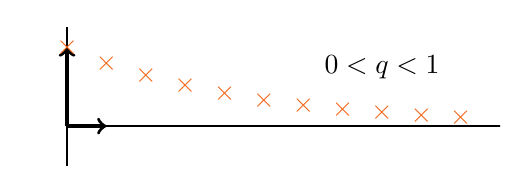
\begin{tikzpicture}[scale=0.5]
\clip (-1,-1) rectangle (11,2.5);
\draw [thick] (0,0)--(22,0);
\draw [thick] (0,-2)--(0,28);
\draw [->, very thick] (0,0)--(1,0);
\draw [->,very thick] (0,0)--(0,2);
\draw (8,1.5) node {$0<q<1$};
\foreach \k in {0,1,...,10} {\draw [ocre, very thick] (\k,{2*0.8^\k}) node {$\times$};}
\end{tikzpicture}

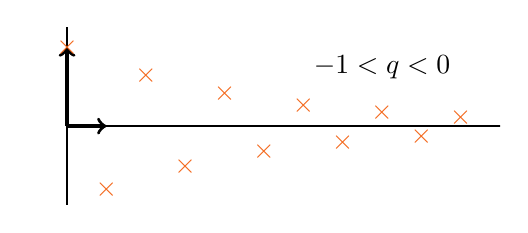
\begin{tikzpicture}[scale=0.5]
\clip (-1,-2) rectangle (11,2.5);
\draw [thick] (0,0)--(22,0);
\draw [thick] (0,-2)--(0,28);
\draw [->, very thick] (0,0)--(1,0);
\draw [->,very thick] (0,0)--(0,2);
\draw (8,1.5) node {$-1<q<0$};
\foreach \k in {0,1,...,10} {\draw [ocre, very thick] (\k,{2*(-0.8)^\k}) node {$\times$};}
\end{tikzpicture}

$\bullet \quad$ Si $q \leqslant -1$, la suite $(q^n)$ n'admet pas de limite.

\end{minipage}

\end{proposition}

\begin{demonstration} Traitons séparément les différents cas mentionnés ici :

\textbf{Premier cas} : $q>1$ :

\vskip60pt

\textbf{Deuxième cas} : $0 < q < 1$

\vskip60pt

\textbf{Troisième cas} : $-1 < q <0$



\newpage

\textbf{Quatrième cas} : $q \leqslant -1$

Dans ce cas, $q^2 \geqslant 1$.
\begin{itemize}
\item D'une part, pour tout entier naturel $k$, $q^{2k}=(q^2)^k$. Ainsi, $\displaystyle \lim_{k \to +\infty} q^{2k} = +\infty$.
\item D'autre part, pour tout entier naturel $k$, $q^{2k+1}=q\times (q^2)^k$. On en déduit que $\displaystyle \lim_{k \to +\infty} q^{2k+1} = -\infty$.
\item Les termes de rangs pairs de la suite $(q^n)$ tendent vers $+\infty$ et les termes de rangs impairs tendent vers $-\infty$. La suite $(q^n)$ ne peut admettre de limite, finie ou infinie.
\end{itemize}\end{demonstration}

\begin{example} On considère la suite géométrique $(u_n)$ de premier terme $u_0=-2$ et de raison $q=4$.
\vskip30pt
\end{example}

\begin{example} Soit $q$ un réel tel que $-1< q < 1$. 

Pour tout entier naturel $n$, on note $u_n=1+q+q^2+q^3+\ldots + q^n = \displaystyle \sum_{k=0}^n q^k$.
\vskip100pt
\end{example}

\begin{example}Pour tout entier naturel $n$, on pose $u_n = \dfrac{1-4^n}{2+3^n}$. 

\vskip100pt
\end{example}


\newpage

\section{Convergence des suites monotones}

\subsection{Théorème de convergence}

\begin{theorem}[Convergence des suites monotones] Soit $(u_n)$ une suite croissante.
\begin{itemize}
\item Si la suite $(u_n)$ est majorée par un réel $M$, alors la suite $(u_n)$ est convergente et $\displaystyle \lim_{n \to +\infty} u_n \leqslant M$.
\item Si la suite $(u_n)$ n'est pas majorée, alors $\displaystyle \lim_{n \to +\infty} = +\infty$.
\end{itemize} \end{theorem}


\begin{demonstration}[Second point uniquement] Supposons que la suite $(u_n)$ ne soit pas majorée. 

\vskip50pt
\end{demonstration}


\textbf{Attention à ne pas dire}, dans le cas où la suite est croissante est majorée par $L$, que la limite vaut $L$ ! \\
Ce raisonnement peut être mis en défaut assez simplement : si une suite est majorée par $L$, alors elle l'est aussi par $L+1$, ce qui signifierait qu'elle tendrait aussi vers $L+1$ ? Le calcul de la limite demandera au moins une étape supplémentaire.


\begin{example} On considère la suite $(u_n)$ définie par $u_0=1$ et, pour tout entier naturel $n$, $u_{n+1}=\dfrac{1}{5}u_n+4$. On peut montrer par récurrence que la suite $(u_n)$ est croissante et que pour tout entier $n$, $u_n \leqslant 5$. On admettra ces deux points pour la suite de l'exemple

Ainsi, la suite $(u_n)$ est croissante et majorée. 

\vskip170pt

\end{example}

\textbf{ Il est important de montrer que la suite converge avant de passer à la limite.} 
 
 En effet, prenons la suite $(v_n)$ définie par $v_0=1$ et pour tout entier $n$, $v_{n+1}=2v_n+3$. D'après le même raisonnement, si $(v_n)$ admet pour limite $\ell$, alors $\ell=2\ell+3$, soit $\ell=-3$... ce qui est absurde : on voit facilement que pour tout entier $n$, $v_n>0$. On a même $\displaystyle \lim_{n \to +\infty} v_n = +\infty$ !

\begin{theorem}[Convergence des suites monotones] Soit $(u_n)$ une suite décroissante.
\begin{itemize}
\item Si la suite $(u_n)$ est minorée par un réel $m$, alors la suite $(u_n)$ est convergente et $\displaystyle \lim_{n \to +\infty} u_n \geqslant m$.
\item Si la suite $(u_n)$ n'est pas minorée, alors $\displaystyle \lim_{n \to +\infty} = -\infty$.
\end{itemize} \end{theorem}


\subsection{Algorithme de seuil}

Lorsqu'une suite est strictement monotone, il est courant de rechercher la valeur à partir de laquelle elle dépassera un certain seuil. Il est possible de résoudre un tel problème à l'aide d'une résolution d'équation ou d'un algorithme.

\begin{example}On considère la suite $(u_n)$ définie par $u_0=9$ et, pour tout entier naturel $n$, $u_{n+1}=\dfrac{u_n}{2}+1$.

On peut montrer, par exemple par récurrence, que cette suite est strictement décroissante et que, pour tout entier naturel $n$, $u_n \geqslant 2$. La suite $(u_n)$ étant décroissante et minorée, on en déduit qu'elle est convergente. Un autre calcul permettra de montrer que $\ell = \displaystyle \lim_{n \to +\infty} u_n=2$.

D'après la définition de la limite, pour tout $\varepsilon >0$, il existe un entier $N$ tel que, pour tout $n>N$, on a $u_n \in ]2-\varepsilon ; 2+\varepsilon [$. La suite $(u_n)$ étant ici décroissante, il suffit de trouver le premier rang $n$ pour lequel $u_n \leqslant 2+\varepsilon$ : les termes suivants seront forcément compris entre 2, qui est la limite, et $2+\varepsilon$.

\begin{itemize}
\item On commence au rang $n=0$ et on prend comme valeur initiale de la suite celle de $u_0$.
\item Tant que la valeur actuelle $u_n$ de la suite est supérieure à $2+\varepsilon$ on calcule la valeur suivante de la suite et on incrémente le rang de 1.
\item Si la valeur actuelle de $u_n$ est inférieure à $2+\varepsilon$, alors on s'arrête ici et on renvoie la valeur du rang $n$.
\end{itemize}

\textbf{Pseudo-algorithme}

\begin{center}
\fbox{\begin{minipage}{0.6\linewidth}Variable d'entrée : $\varepsilon$ \\
$U = 9$\\
$N=0$\\
Tant que $U > 2+\varepsilon$\\
\indent  $\quad U \leftarrow U/2+1$\\
\indent $\quad N \leftarrow N+1$\\
Fin Tant que\\
Renvoyer $N$\end{minipage}
}
\end{center}

La valeur de $n$ est stockée dans la variable $N$ et celle de $u_n$ est stockée dans la variable $U$. A chaque étape, le terme suivant de la suite est calculé : $N$ est augmenté de 1 et on applique la relation de récurrence de la suite $(u_n)$ pour mettre à jour la valeur de $U$. Le programme renvoie alors la première valeur de $n$ telle que $u_n$ n'est pas strictement supérieur à $2+\varepsilon$. On peut alors construire une fonction en Python qui prend en paramètres un réel $E$ positif ou nul et qui renvoie cet entier $n$.

\begin{lstlisting}[language=python]
def seuil(E):
	U = 9
	N = 0
	while U > 2 + E:
		U = U/2 + 1
		N = N + 1
	return N
\end{lstlisting}

Dans notre cas, l'exécution de l'instruction \textbf{seuil(0.001)} renvoie la valeur 13. Cela signifie que $u_{13}$ est le premier terme de la suite inférieur ou égal à 2.001.\end{example}

Cet algorithme peut varier sur certains aspects : on peut par exemple avoir une suite croissante, auquel cas on souhaitera le premier terme supérieur à une valeur donnée. On peut également donner en entrée la valeur à franchir plutôt que la différence entre la limite et les valeurs des termes de la suite. Cependant, la construction d'un tel algorithme est toujours la même.


















\end{document}